\documentclass[tikz,border=2pt]{standalone}
\usepackage{amsmath,amssymb}
\usepackage{tikz}
\usetikzlibrary{arrows.meta,matrix}

\begin{document}
% Entry (i, j) of AB is row i of A dotted with column j of B; sizes must chain:
% (m x n)(n x k) = m x k.
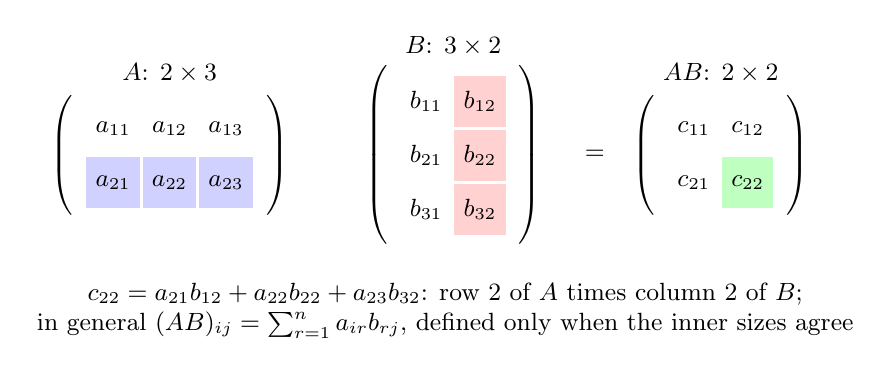
\begin{tikzpicture}[every node/.style={font=\small}]
	\matrix (A) [matrix of math nodes, nodes={minimum size=6.5mm, anchor=center}, left delimiter=(, right delimiter=), column sep=1pt, row sep=1pt] at (0,0) {
		a_{11} & a_{12} & a_{13} \\
		|[fill=blue!18]| a_{21} & |[fill=blue!18]| a_{22} & |[fill=blue!18]| a_{23} \\
	};
	\matrix (B) [matrix of math nodes, nodes={minimum size=6.5mm, anchor=center}, left delimiter=(, right delimiter=), column sep=1pt, row sep=1pt] at (3.6,0) {
		b_{11} & |[fill=red!18]| b_{12} \\
		b_{21} & |[fill=red!18]| b_{22} \\
		b_{31} & |[fill=red!18]| b_{32} \\
	};
	\node at (5.4,0) {$=$};
	\matrix (C) [matrix of math nodes, nodes={minimum size=6.5mm, anchor=center}, left delimiter=(, right delimiter=), column sep=1pt, row sep=1pt] at (7.0,0) {
		c_{11} & c_{12} \\
		c_{21} & |[fill=green!25]| c_{22} \\
	};
	\node[anchor=south, font=\small] at (A.north) {$A$: $2\times3$};
	\node[anchor=south, font=\small] at (B.north) {$B$: $3\times2$};
	\node[anchor=south, font=\small] at (C.north) {$AB$: $2\times2$};
	\node[anchor=north, align=center] at (3.5,-1.5) {$c_{22}=a_{21}b_{12}+a_{22}b_{22}+a_{23}b_{32}$: row $2$ of $A$ times column $2$ of $B$;\\ in general $(AB)_{ij}=\sum_{r=1}^{n}a_{ir}b_{rj}$, defined only when the inner sizes agree};
\end{tikzpicture}
\end{document}
